Because using more partitions did not improvement the learned preconditioners, we will now test with a smaller number of partitions. The partition count we will use in this test is \(\{1,2,3,4,5\}\) and that is the only difference between the runs. With the 200 base learning iterations to make the results comparable with the previous test with more partitions.


\begin{figure}[H]
    \begin{minipage}{.49\textwidth}
        \center
        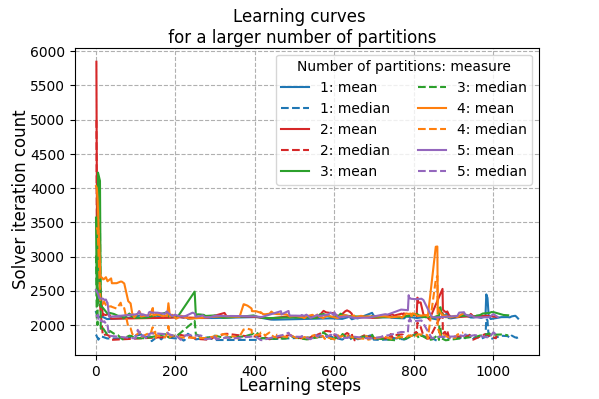
\includegraphics[width=1\textwidth]{plots/fewer_num_par_learning_curve.png}
        \caption{Learning curves for the testing with fewer number of partition, with the same structure as figure \ref{fig: more par learning curves}.\\}
        \label{fig: fewer par learning curves}
    \end{minipage}
    \begin{minipage}{.02\textwidth}
        
    \end{minipage}
    \begin{minipage}{.49\textwidth}
        \center
        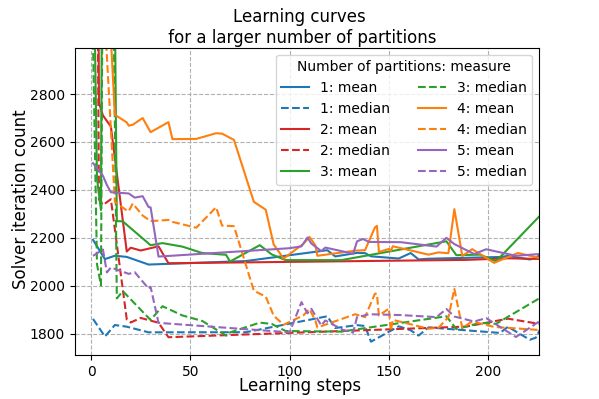
\includegraphics[width=1\textwidth]{plots/fewer_num_par_learning_curve_zoom.png}
        \caption{Learning curves for the test with fewer number of partition, the same data as figure \ref{fig: fewer par learning curves}, but zoomed in to the lower left corner to see the initial learning.}
        \label{fig: fewer par learning curves zoom}
    \end{minipage}
\end{figure}

The learning curves, seen in figures \ref{fig: fewer par learning curves} and \ref{fig: fewer par learning curves zoom}, are as excepted with fewer partitions has faster learning and it plateaus almost immediately. With the slowest run being with 4 partitions, orange learning curve, plateauing at the 100th learning step. The problem where accepting a worse state and not being able to get back to a similar solver iteration counts does not happen for these runs, as can be seen a bit after the 800th learning step, there is a major spike in solver iteration counts but all tests get back to previous iteration counts at around iteration 900. 

In the evaluation of the learned preconditioners, figure \ref{fig: fewer par test measure} and \ref{fig: fewer par BvJ}, we can see that they are all on par or slightly better than Jacobi preconditioning for all three measure. With using 1 partition begin best in this seed.


\begin{figure}[H]
    \begin{minipage}{.49\textwidth}
        \center
        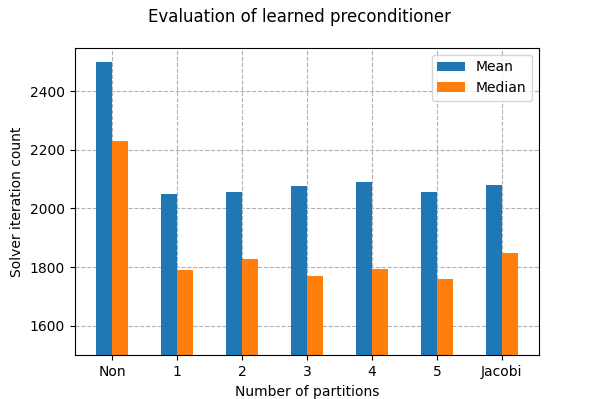
\includegraphics[width=1\textwidth]{plots/fewer_num_par_test_measure.png}
        \caption{Mean and median solver iteration count from the evaluate of the 5 learned preconditioners. The plot has the same structure as figure \ref{fig: more par test measure}.\\}
        \label{fig: fewer par test measure}
    \end{minipage}
    \begin{minipage}{.02\textwidth}
        
    \end{minipage}
    \begin{minipage}{.49\textwidth}
        \center
        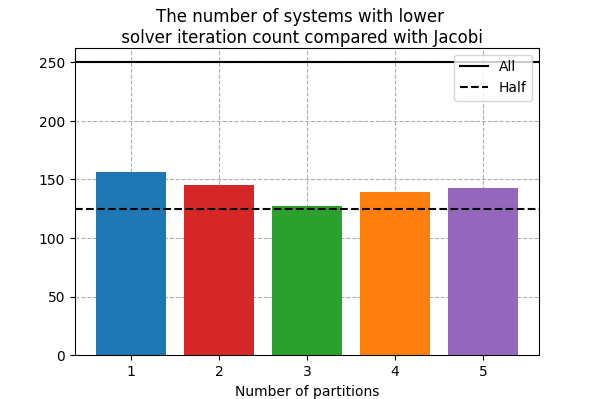
\includegraphics[width=1\textwidth]{plots/fewer_num_par_BvJ.png}
        \caption{Individual linear system comparison between the learned preconditioners and the Jacobi preconditioner. The plot has the same structure as figure \ref{fig: more par BvJ}.}
        \label{fig: fewer par BvJ}
    \end{minipage}
\end{figure}

The coefficients of the learned preconditioners with fewer number partitions, table \ref{tabel: fewer par coefficients}, are not equal, because of the inheritant randomness of the algorithm, but the values are close with an average value of \(-0.013641246\) and standard deviation of \(0.00445245\). Because of this and the increased speed in learning. The new standard preconditioner will have 1 partition in the superdiagonal.


\begin{table}[H]
    \center
    \begin{tabular}{|r|l|}
        \hline
        Par & Partition coefficients \\ \hline
        1 &\([-0.01463557]\) \\
        2 &\([-0.01678746, -0.02122048]\) \\
        3 &\([-0.00676193, -0.01237617, -0.01208201]\) \\
        4 &\([-0.02033992, -0.01883074, -0.01200618, -0.01339265]\)\\
        5 &\([-0.01600863, -0.00575484, -0.00860635, -0.01501886, -0.0107969]\) \\ \hline
    \end{tabular}
    \caption{Table of the learned preconditioners coefficients, with a row for each different number of partitions.}
    \label{tabel: fewer par coefficients}
\end{table}

From both of the test with changing the number of partitions we did not solve the problem of the preconditioner plateauing, as was the intention with the tests, but we did confirm that using more partitions would result in slower learning, to the point of a good preconditioner being unlearnable, and with fewer learning faster and plateauing quickly. 